\chapter{KITTI Dataset}
\label{cha:KITTI Dataset}

\begin{FraseCelebre}
  \begin{Frase}
    Texto.
  \end{Frase}
  \begin{Fuente}
    Autor texto
  \end{Fuente}
\end{FraseCelebre}

\noindent
La gran mayoría de sistemas de visión por computador basan sus arquitecturas en modelos de Deep Learning, dichos modelos se han probado a lo largo de la última década como aquellos con la capacidad de extraer a partir de los sensores utilizados la mayor cantidad de información del entorno que nos rodea. El mayor problema en la creación de estos modelos es la necesidad de grandes fuentes de datos que permitan el entrenamiento y evaluación de dichos modelos, ya que para la obtención de los datos solo el necesaria la grabación de los datos de los sensores, pero la obtención de la información a inferir o ground-truth necesita de la anotación a mano de los datos dados por los sensores.

En el caso de los sistemas de conducción autónomos, el desarrollo de este tipo de sistemas de percepción parte de múltiples centros de investigación y empresas eligen su propio sistema de conducción base con el cual se graba la información de los sensores y posteriormente de anota a mano los datos recabados para poner entrenar a los algoritmos en las tareas que se requieran. En el caso de este trabajo, se utilizará el dataset de KITTI ya que es aquel que más se asemeja al vehículo \ac{T4AC} del grupo de investigación RobeSafe, ya que como se comenta en el Capítulo \ref{cha:Propuesta de trabajo}, es aquel vehículo en el que se pretende que se pueda utilizar el sistema de percepción a construir.

\section{Elección del dataset}
\label{sec:Elección del dataset}

La elección de un dataset con el que trabajar, define en cierta manera la construcción de los algoritmos que pueden ser construidos si se utiliza únicamente una fuente de datos. En el campo de la conducción autónoma se tienen multitud de datasets que permiten la creación de sistemas de percepción, entre los más famosos encontramos: KITTI dataset \cite{kitti_dataset} desarrollado en el \ac{KIT} en Alemania, nuScenes \cite{nuscenes_dataset} creada por la empresa norteamericana nuTonomy o Waymo Open Dataset \cite{waymo_dataset} creado por la empresa Waymo (antiguo proyecto de vehículo autónomo de Google) perteneciente al gigante Alphabet. Estos dataset no solo se diferencian por el vehículo utilizado con el que se ha obtenido dicho dataset, sino también por el conjunto de sensores utilizados, la cantidad y variedad de escenas, además de los diferentes tipos de ground-truth que se encuentran dentro de estos. A continuación se presentan las diferencias y similitudes entre los vehículos del grupo RobeSafe y el vehículo utilizado en el dataset de KITTI, para comprender la elección del dataset de KITTI.

\subsection{Vehículo del proyecto T4AC}
\label{sec:Vehículo del proyecto T4AC}

El vehículo diseñado en el grupo de investigación RobeSafe dentro del proyecto \acl{T4AC}, se utiliza como base en la que probar los modelos y algoritmos de conducción autónoma, tras haber sido estos diseñados y probados en el simulador de conducción autónoma CARLA \cite{carla}. Este vehículo se encuentra basado en el chasis TABBY EVO al ser esta una plataforma Open-Source sobre la que poder aportar a su desarrollo, tal y como se muestra en la Figura \ref{fig:Vehículo T4AC} donde se observa el avance sobre el diseño de la plataforma base. 

\begin{figure}[H]
	\begin{minipage}{0.48\textwidth}
		\centering
		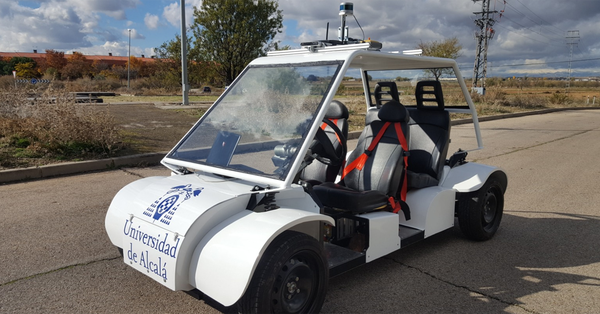
\includegraphics[width=1\linewidth]{Book/figures/4_kitti/vehiculo_t4ac.png}
		\caption{Vehículo T4AC}
		\label{fig:Vehículo T4AC}
	\end{minipage}\hfill
	\begin{minipage}{0.48\textwidth}
		\centering
		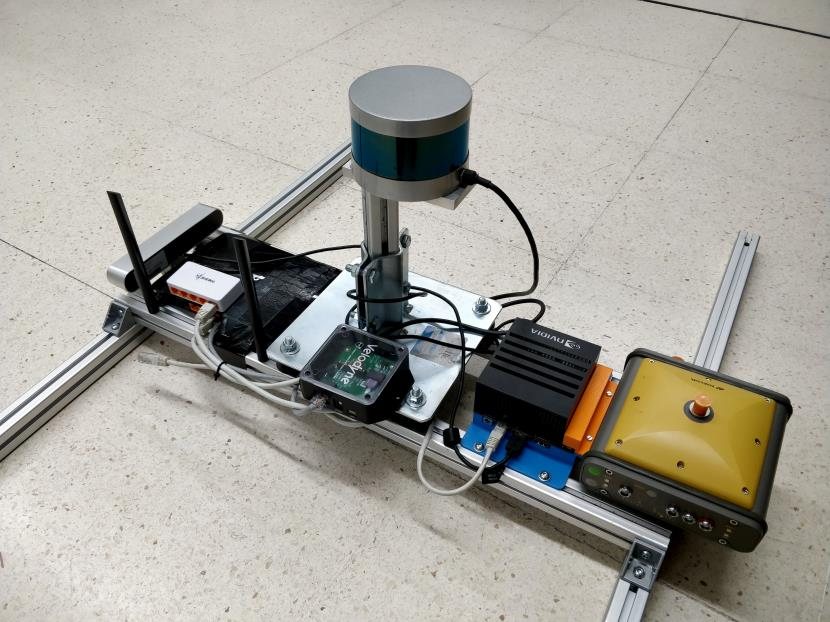
\includegraphics[width=0.7\linewidth]{Book/figures/4_kitti/chasis_hardware.png}
		\caption{Chasis con el hardware utilizado en el vehículo T4AC}
		\label{fig:Chasis con el hardware utilizado en el vehículo T4AC}
	\end{minipage}
\end{figure}

En cuanto al desarrollo de este trabajo, el apartado más importante de este vehículo consiste en la suite de sensores con el que cuenta el automóvil. Gran parte del sistema de sensores integrados en el vehículo se encuentra en montado en el chasis de la Figura \ref{fig:Chasis con el hardware utilizado en el vehículo T4AC}, de forma global por tanto, el vehículo se encuentra compuesto por:

\begin{itemize}
    \item Un sistema mundial de navegación por satélite o \acs{GNSS} en el que se aplican técnicas de posicionamiento global diferencial para mejorar la precisión del posicionamiento del vehículo.
    \item Un sistema de odometría basado en encoders construido sobre las ruedas traseras para el cálculo del movimiento del vehículo.
    \item Un \ac{LiDAR} de 128 haces capaz de generar 2.400.000 puntos por segundo, modelo Velodyne VLS-128.
    \item Un sistema de visión estereoscópica, modelo ZED de StereoLabs.
\end{itemize}

En el capítulo siguiente se comprenderá la gran similitud en cuanto a sensores que tiene este vehículo en relación al utilizado en el \ac{KIT} para la construcción del dataset de KITTI.

\subsection{Vehículo del dataset KITTI}
\label{sec:Vehículo del dataset KITTI}

El vehículo utilizado en el dataset de KITTI se encuentra basado en un Volkswagen CC sobre el que se ha montado una serie de sensores con los que obtener los suficientes datos con los que comprender de forma correcta el entorno del vehículo. Dicho vehículo consta de un sistema de sensores compuesto por los siguiente componentes:

\begin{itemize}
    \item Un sistema de posicionamiento global o \acs{GPS} junto con un sistema de medición inercial o \acs{IMU}, sobre los que se aplican técnicas de posicionamiento global diferencial con los que calcular la posición global del vehículo según se desplaza.
    \item Un \ac{LiDAR} de 64 haces capaz de generar 1.200.000 puntos por segundo, modelo Velodyne HDL-64E.
    \item Dos sistemas de visión estereoscópica, siendo uno de ellos en escala de grises y el otro en formato RGB (que muestra muestra los diferentes colores). Las cuatro cámaras constan de resolución de 1392x512 píxeles con un \ac{FoV} vertical de 35º y horizontal de 90º, tomadas a una velocidad de 10 Hz.
\end{itemize}

Los sensores montados en este vehículo como se ha presentado y se muestra en el Figura \ref{fig:Vehiculo_utilizado_en_kitti}, son muy similares a los utilizados en el vehículo T4AC. En este trabajo solo se pretende utilizar una cámara monocular junto un \ac{LiDAR}, para ello en el caso de KITTI se utilizará el unico \ac{LiDAR} a bordo del vehículo, además de la cámara 2 del vehículo que como se observa en la Figura \ref{fig:Medidas_del_vehiculo_utilizado_en_kiti}, es aquella que tiene un formato RGB además de encontrarse más centrada en relación al propio centro del vehículo.

\begin{figure}[H]
	\begin{minipage}{0.48\textwidth}
		\centering
		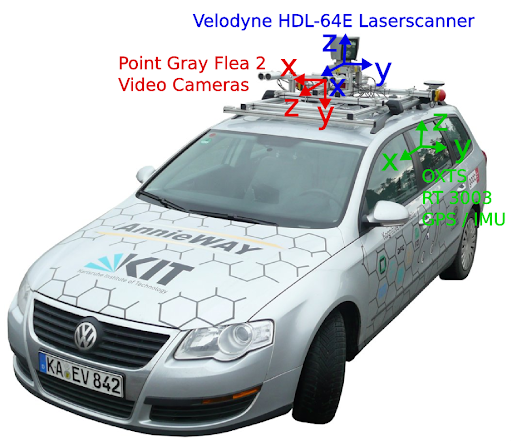
\includegraphics[width=0.8\linewidth]{Book/figures/4_kitti/kittis_car.png}
		\caption{Vehículo utilizado en KITTI.}
		\label{fig:Vehiculo_utilizado_en_kitti}
	\end{minipage}\hfill
	\begin{minipage}{0.48\textwidth}
		\centering
		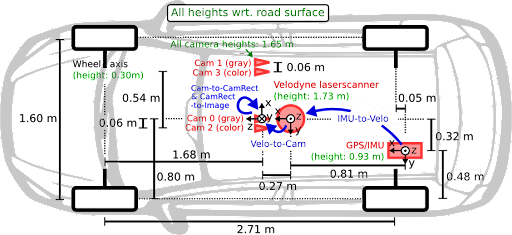
\includegraphics[width=1\linewidth]{Book/figures/4_kitti/kittis_car_measures.png}
		\caption{Medidas del vehículo utilizado en KITTI}
		\label{fig:Medidas_del_vehiculo_utilizado_en_kiti}
	\end{minipage}
\end{figure}

Mientras que la elección del dataset del KITTI es muy importante por la similitud en cuanto a los diferentes sensores que este tiene con el vehículo T4AC es muy importante tener en cuenta las pequeñas diferencias que podemos encontrar, como la diferencia en resolución y \ac{FoV} de la cámara a utilizar además de la diferencia en traslación y rotación entre ambos sensores. Esto es importante ya que para poder pasar de un vehículo a otro, el sistema a construir debe de ser invariante a estas características, ya que no es algo sencillo y es parte fundamental de este trabajo.

\section{Contenido del dataset}
\label{sec:Contenido del dataset}

En 2012 los sistemas de visión artificial eran raramente utilizados en aplicaciones robóticas reales. Una de las razones por la que esto sucedía, era por la falta de datos de prueba de referencia con los que imitar a las situaciones con las que se puede encontrar un robot. En este momento el \ac{KIT} publica su dataset KITTI, en dicho datase se presenta su plataforma de conducción autónoma, presentada en el capítulo anterior, junto con varios conjuntos de datos anotados con los que poder desarrollar diferentes algoritmos de percepción.

En cuanto a la información proporcionada por el dataset, como se puede esperar, se proporciona todo aquella información grabada por los sensores en las diferentes escenas anotadas. Por lo que entre la información dada se encuentra:

\begin{itemize}
    \item Las imágenes sincronizadas y sin sincronizar, rectificadas y sin rectificar, de las 4 cámaras de ambos sistemas estereoscópicos del vehículo.
    \item Las nubes de puntos obtenidas del \ac{LiDAR} y guardadas como ficheros en binario.
    \item La localización, velocidad, aceleración junto con la información del \ac{GPS} y la \ac{IMU} del vehículo.
    \item Las matrices de calibración de las cámaras junto con las matrices de transformación entre los diferntes sensores.
\end{itemize}

A partir de los datos recabados de todos los sensores se han definidos diferentes retos a completar, para cada uno de ellos se han generado anotaciones sobre las cuales diseñar los algoritmos que resuelvan las diferentes tareas, las cuales son mayoritariamente de percepción. Entre las diferentes tareas que trata de resolver KITTI con su gran cantidad de datos se encuentran las siguientes:

\begin{itemize}
    \item Evaluación del flujo de la escena, para la obtención del movimiento de los objetos del entorno a partir de las imágenes de las cámaras.
    \item Estimación de la profundidad, para la incorporación de una nueva dimensión sobre las imágenes de las cámaras.
    \item Odometría visual y evaluación SLAM, para la reducción del error cometido con el \ac{GPS} y la \ac{IMU} a partir del uso de cámaras.
    \item Detección de objetos 2D, 3D y en \ac{BEV}, para la localización de los objetos del entorno en relación al propio vehículo.
    \item Seguimiento de objetos, para la obtención de la localización de los objetos a partir de secuencias completas del trayecto de un vehículo.
    \item Detección de carriles, para la comprensión del terreno por el cual el vehículo es capaz de conducir.
    \item Segmentación semántica, para la detección de los objetos del entorno a nivel de píxel sobre las cámaras.
\end{itemize}

Debido a la gran cantidad de datos que ofrece el dataset de KITTI, gran parte de la comunidad científica se ha volcado en su estandarización como medio de comparación de diferentes algoritmos. Hasta hace un par de años, la gran mayoría de papers de visión artificial utilizaban este dataset para mostrar su precisión en los escenarios ofrecidos, pero con la aparición de nuevos dataset como el Waymo Open dataset \cite{waymo_dataset} o el dataset de nuScenes \cite{nuscenes_dataset} se comienza a dejar de utilizar tanto este dataset a favor de aquellos con más cantidad de datos y escenarios además de sistemas de sensores más actualizados.

\begin{figure}[H]
    \centering
    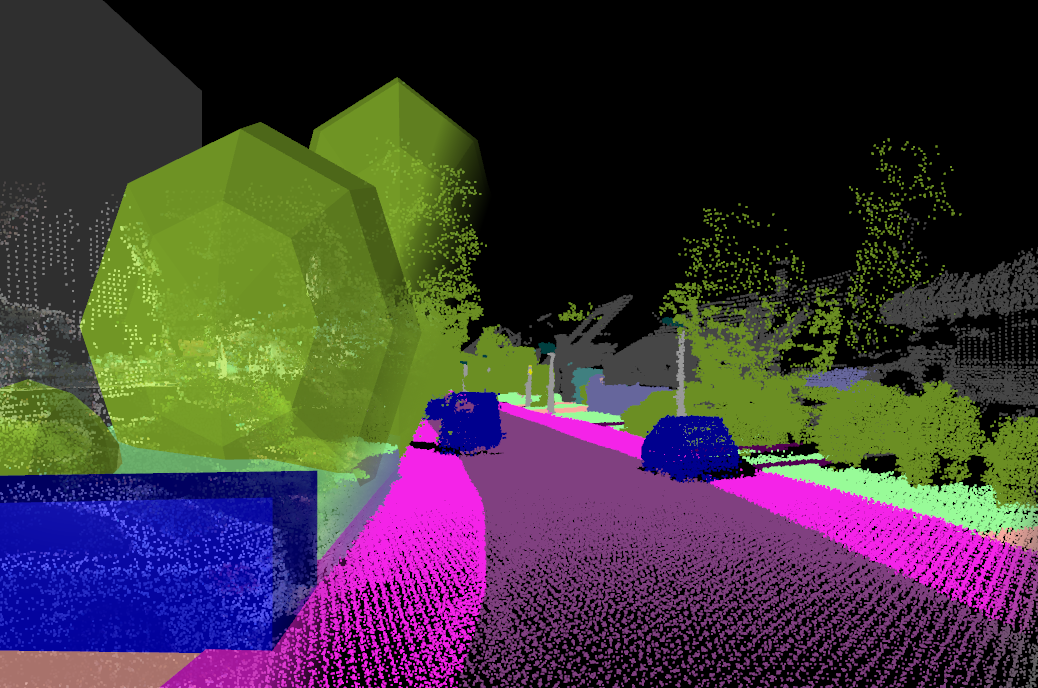
\includegraphics[width=0.55\textwidth]{Book/figures/4_kitti/kitti360_pcl.png}
    \caption{Nube de puntos segmentada en KITTI-360.}
    \label{fig:Nube de puntos segmentada en KITTI-360.}
\end{figure}

Uno de los mayores problemas con este dataset, recae en la falta de herramientas oficiales que ayuden en su utilización. Mientras que en 2012 aun no se habían definido las técnicas basadas en Deep Learning como aquellas con un mayor potencial en la explicabilidad del entorno, se diseñó únicamente una pequeña herramienta de trabajo en MATLAB que hoy en día está bastante anticuada, debido al gran uso de Python por frameworks de Deep Learning como Pytorch \cite{Pytorch} o Tensorflow \cite{Tensorflow}. Esto es solucionado mediante la creación de herramientas propias, o mediante el uso de herramientas de código libre (open source) creadas por la comunidad científica.

Debido a la gran importancia a lo largo de los años del dataset de KITTI, no solo en cantidad de citas en diversos artículos científicos, sino a nivel del desarrollo de nuevas técnicas que han producidos avances en este campo, en 2021 se presentó KITTI-360 \cite{KITTI-360}. Esta nueva versión del dataset trata de eliminar ciertas limitaciones del dataset original, como la generación de anotaciones en 360º y no solo la parte frontal del vehículo, la creación de nuevas tareas y anotaciones como la segmentación semántica de la nube de puntos, tal y como se en la Figura \ref{fig:Nube de puntos segmentada en KITTI-360.}, o la adicción de diferentes condiciones climáticas y gran cantidad de nuevos escenarios.
